\chapter{Opis projektnog zadatka}
		%nas sadrzaj
		Cilj ovog projekta je razviti web aplikaciju „DentAll“ kojom će pružatelji usluga zdravstvenog turizma moći evidentirati i koordinirati lokalni smještaj i prijevoz korisnika usluga. Time bi se zdravstveni turizam učinio privlačnijim rješavanjem brige i cijene smještaja i prijevoza korisnika pri njihovom obitavanju u mjestu gdje koriste spomenute usluge. Uz to bi klijenti pružatelja usluga bili u mogućnosti unaprijed vidjeti geografsku sliku smještaja i okolice te moguće turističke opcije i kretanja tijekom privremenog obitavanja .
		
		\smallskip
		Aplikacija bi olakšala brige vlasnika usluga zdravstvenog turizma evidentiranjem, organizacijom i praćenjem smještaja i prijevoza klijenata uz programsku podršku interneta. Time se nastoji nadomjestiti nedostatak ovisnosti pružatelja zdravstvenih usluga o raznim i višestrukim pružateljima smještajnih usluga. Takvim pristupom kroz javnu i lagano dostupnu uslugu smanjio bi se broj posrednika u organizaciji i administraciji pružanja usluga zdravstvenog turizma. Također bi klijenti pronalazili sve potrebne informacije oko odabranog zdravstvenog turizma, tj. uz same zdravstvene usluge i o smještaju te prijevozu za svaki termin, čineći sam odabir prisustvovanja u inozemnim zdravstvenim uslugama jednostavniji i privlačniji.
		
		\smallskip
		Trenutna postojeća rješenja uključuju korištenje hotela i motela, što čini cijeli proces zdravstvenog turizma skupljim i kompliciranijim. Dugoročno bi pružateljima bilo isplativije iznajmljivati vlastite nekretnine u sklopu pružanja cjelokupnih usluga. Također je u trenutnim rješenjima prijevoz ostavljen na odgovornost klijenata, što otežava korištenje cijele usluge i njezinu privlačnost. Spajanjem oba problema u jedan sustav bi učinilo uslugu zdravstvenog turizma puno efektivnijom i jeftinijom, a time i više privlačnom mogućim budućim klijentima.
		
		\smallskip
		\noindent Postojeće vrste konkurentnih rješenja:
		\begin{packed_item}
			\item  javno dostupne informacije o načinima sudjelovanja u zdravstvenom turizmu i pripadnim članovima
			\item  udruge sa svrhom spajanja svih dionika pružanja usluga zdravstvenog turizma
		\end{packed_item}
		
		\break
		\begin{wrapfigure}{r}{6cm}
			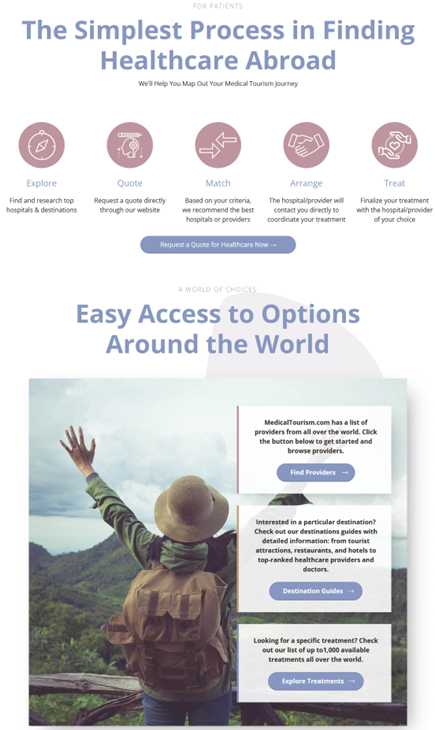
\includegraphics[width=6cm]{slike/konkurencija.png} %veličina slike u odnosu na originalnu datoteku i pozicija slike
			\caption{Mogućnosti povezivanja klijenata i pružatelja koje nudi web stranica "MedicalTourism.com"}
			\label{fig:konkurencija}
			\centering
		\end{wrapfigure}
		
		Primjer za usluge pružanja informacija je web stranica „MedicalTourism.com“ koja pruža korisnicima podatke o pružateljima zdravstvenih usluga, smještaja i mogućih tretmana koje spomenute usluge pružaju. Također sadrži i mnoge druge informacije kao vodiče za destinacije, usporedbe cijena i slično. No ipak je spomenuta web aplikacija napravljena za pružanje laganog pristupa svim potrebnim informacijama za moguće klijente, pružatelje zdravstvenih usluga, pružatelje smještaja te osiguravajuća društva na jednom mjestu te se time ne sukobljava do konkurentske razine sa svrhom kreiranja projektne aplikacije.
		
		
		Dok je primjer druge vrste rješenja, čak konkurentnije ideji projekta, udruga Medical Tourism Association, koja spaja sve potrebne članove zdravstvenog turizma kroz program članstva. Udruga operira po cijelom svijetu i služi svrhu omogućavanja pružanja usluga zdravstvenog turizma kroz povezivanje potrebnih članova te svrhu informiranja javnosti o mogućnostima korištenja tih usluga. Također podržava edukaciju budućih pružatelja sa sveukupnim ciljem povećanja učestalosti zdravstvenog turizma u svijetu. Ovdje opisan projekt ipak sadrži određene funkcionalnosti koje nedostaju navedenoj konkurenciji, kao automatiziran proces organizacije i administracije, te lagano dostupni pregled informacija o obitavanju za klijente zdravstvenih usluga.
		
		
		%\begin{figure}[H]
		%	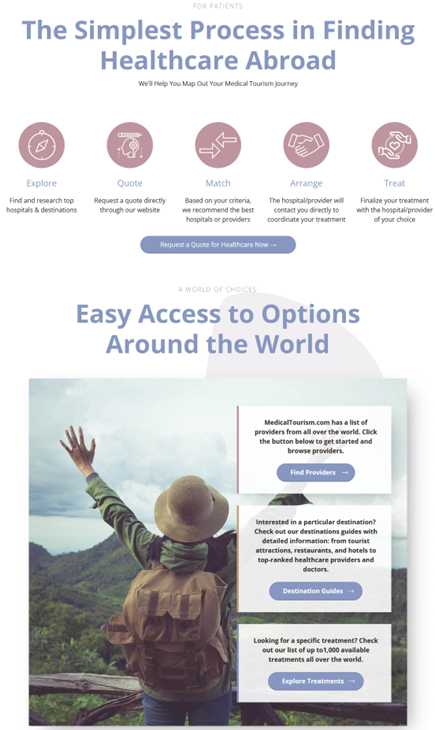
\includegraphics[scale=0.4]{slike/konkurencija.png} %veličina slike u odnosu na originalnu datoteku i pozicija slike
		%	\raggedleft
		%	\caption{Prikaz procesa i mogućnosti usluga povezivanja klijenata i pružatelja usluga koju nudi web stranica "MedicalTourism.com"}
		%	\label{fig:konkurencija}
		%\end{figure}
		
		
		\break
		Ciljani klijenti opisanih usluga su pružatelji usluga zdravstvenog turizma po cijelom svijetu, uključujući Hrvatsku i slične države sa jeftinom cijenom boravka. Optimalno bi bilo započeti pružanje usluga aplikacije najprije Europskim državama i okolici, a zatim, uz dovoljnu uspješnost i isplativost projekta, raširiti dostupnost usluge ostatku svijeta. Ciljani klijenti bi također bili i pružatelji lokalnih prijevoznih usluga, od privatnih firmi do javnih taksija, koje bi aplikacija spajala sa pružateljima zdravstvenih usluga za dogovor o prijevozu njihovih klijenata. Također bi, u manjoj perspektivi, evidencija većine korisnika zdravstvenog turizma na jednom mjestu olakšala statističke analize razvoja zdravstvenog turizma po cijelom svijetu.
		
		\medskip
		U aplikaciji postoje četiri uloge:
		\begin{packed_item}
			\item  smještajni administrator
			\item  administrator prijevoznih usluga
			\item  korisnički administrator
			\item  obični korisnik (pacijent)
		\end{packed_item}
		
		Jedan korisnik može imati više administratorskih uloga, dok uloga smještajnog administratora sadrži najveće ovlasti kojima mogu definirati druge korisnike i dodjeljivati uloge. Svaka uloga administratora sadrži određene posebne mogućnosti dodavanja i promjene informacija.
		
		\smallskip
		Smještajni administratori upravljaju podatcima o smještaju; unose podatke o raspoloživom smještaju te definiraju smještajne kapacitete i unose ili brišu osnovne podatke o smještaju. Podatci smještaja se sastoje od tipa stana, kategorije opremljenosti, adrese i vremenskog perioda dostupnosti za korištenje. Uz svaki smještaj je dostupan grafički prikaz geografskog položaja uz Google Maps usluge.
		
		Administratori prijevoznih usluga upravljaju podatcima o prijevoznicima. To uključuje osnovne osobne i kontaktne podatke prijevoznika, vrstu i kapacitet prijevoznog sredstva te radno vrijeme raspoloživosti. Osnovni podatci prijevoznika se ne mogu mijenjati.
		
		Korisnički administratori definiraju korisnike medicinskih usluga uz unos njihovih osnovnih podataka. Podatci korisnika se sastoje od imena, prezimena, kontaktnih podataka, vremena dolaska i odlaska u/iz zemlje te preferencije o veličini i kvaliteti smještaja. Detalji njihovih tretmana se preuzimaju iz vanjske aplikacije o evidenciji medicinskih usluga.

		\break
		Aplikacija periodički provjerava status unesenih podataka i pridjeljuje adekvatni smještaj upisanim korisnicima te po zaključenju plana medicinskih usluga određenog korisnika im pridjeljuje prijevoznike od raspoloživih za svaki od termina. Sa završetkom spomenutog zaključenja sustav šalje poruku elektroničke pošte korisniku medicinskih usluga sa svim potrebnim informacijama te također šalje poruke elektroničke pošte prijevoznicima pridijeljenima terminima korisnika sa svim njima potrebnim informacijama.
		
		\medskip
		Moguće dodatne funckionalnosti za aplikaciju koje se mogu nadodati nakon izvršavanja jezgrenih funkcionalnosti su:
		\begin{packed_item}
			\item  prijavljivanje samog korisnika medicinskih usluga u aplikaciju čime mogu provjeriti osobne podatke, smještaj, prijevoznike i termine
			\item  proširenje aplikacije u dodatnu svrhu prikaza općenitih podataka o medicinskim turizmo za privlačenje dodatnih, klijenata
			\item  mogućnost pridjeljivanja istog smještaja većem broju pacijenata u slučaju da je smještaj dovoljno velik.
		\end{packed_item}
		\break
		%
		
		
		
		%template
		\section{Upute za opis}
		\textit{Na osnovi projektnog zadatka detaljno opisati korisničke zahtjeve. Što jasnije opisati cilj projektnog zadatka, razraditi problematiku zadatka, dodati nove aspekte problema i potencijalnih rješenja. Očekuje se minimalno 3, a poželjno 4-5 stranica opisa.	Teme koje treba dodatno razraditi u ovom poglavlju su:}
		\begin{packed_item}
			\item \textit{potencijalna korist ovog projekta}
			\item \textit{postojeća slična rješenja (istražiti i ukratko opisati razlike u odnosu na zadani zadatak). Dodajte slike koja predočavaju slična rješenja.}
			\item \textit{skup korisnika koji bi mogao biti zainteresiran za ostvareno rješenje.}
			\item \textit{mogućnost prilagodbe rješenja }
			\item \textit{opseg projektnog zadatka}
			\item \textit{moguće nadogradnje projektnog zadatka}
		\end{packed_item}
		
		\textit{Za pomoć pogledati reference navedene u poglavlju „Popis literature“, a po potrebi konzultirati sadržaj na internetu koji nudi dobre smjernice u tom pogledu.}
		\eject
		
		%ostavio za lakše modificiranje ostatka dokumenta
		\section{Primjeri teksta u \LaTeX u}
		
		\textit{Ovo potpoglavlje izbrisati.}\\

		U nastavku se nalaze različiti primjeri kako koristiti osnovne funkcionalnosti \LaTeX a koje su potrebne za izradu dokumentacije. Za dodatnu pomoć obratiti se asistentu na projektu ili potražiti upute na sljedećim web sjedištima:
		\begin{itemize}
			\item Upute za izradu diplomskog rada u \LaTeX u - \url{https://www.fer.unizg.hr/_download/repository/LaTeX-upute.pdf}
			\item \LaTeX\ projekt - \url{https://www.latex-project.org/help/}
			\item StackExchange za Tex - \url{https://tex.stackexchange.com/}\\
		
		\end{itemize} 	


		
		\noindent \underbar{podcrtani tekst}, \textbf{podebljani tekst}, 	\textit{nagnuti tekst}\\
		\noindent \normalsize primjer \large primjer \Large primjer \LARGE {primjer} \huge {primjer} \Huge primjer \normalsize
				
		\begin{packed_item}
			
			\item  primjer
			\item  primjer
			\item  primjer
			\item[] \begin{packed_enum}
				\item primjer
				\item[] \begin{packed_enum}
					\item[1.a] primjer
					\item[b] primjer
				\end{packed_enum}
				\item primjer
			\end{packed_enum}
			
		\end{packed_item}
		
		\noindent primjer url-a: \url{https://www.fer.unizg.hr/predmet/proinz/projekt}
		
		\noindent posebni znakovi: \# \$ \% \& \{ \} \_ 
		$|$ $<$ $>$ 
		\^{} 
		\~{} 
		$\backslash$ 
		
		
		\begin{longtblr}[
			label=none,
			entry=none
			]{
				width = \textwidth,
				colspec={|X[8,l]|X[8, l]|X[16, l]|}, 
				rowhead = 1,
			} %definicija širine tablice, širine stupaca, poravnanje i broja redaka naslova tablice
			\hline \SetCell[c=3]{c}{\textbf{naslov unutar tablice}}	 \\ \hline[3pt]
			\SetCell{LightGreen}IDKorisnik & INT	&  	Lorem ipsum dolor sit amet, consectetur adipiscing elit, sed do eiusmod  	\\ \hline
			korisnickoIme	& VARCHAR &   	\\ \hline 
			email & VARCHAR &   \\ \hline 
			ime & VARCHAR	&  		\\ \hline 
			\SetCell{LightBlue} primjer	& VARCHAR &   	\\ \hline 
		\end{longtblr}
		

		\begin{longtblr}[
				caption = {Naslov s referencom izvan tablice},
				entry = {Short Caption},
			]{
				width = \textwidth, 
				colspec = {|X[8,l]|X[8,l]|X[16,l]|}, 
				rowhead = 1,
			}
			\hline
			\SetCell{LightGreen}IDKorisnik & INT	&  	Lorem ipsum dolor sit amet, consectetur adipiscing elit, sed do eiusmod  	\\ \hline
			korisnickoIme	& VARCHAR &   	\\ \hline 
			email & VARCHAR &   \\ \hline 
			ime & VARCHAR	&  		\\ \hline 
			\SetCell{LightBlue} primjer	& VARCHAR &   	\\ \hline 
		\end{longtblr}
	


		
		
		%unos slike
		\begin{figure}[H]
			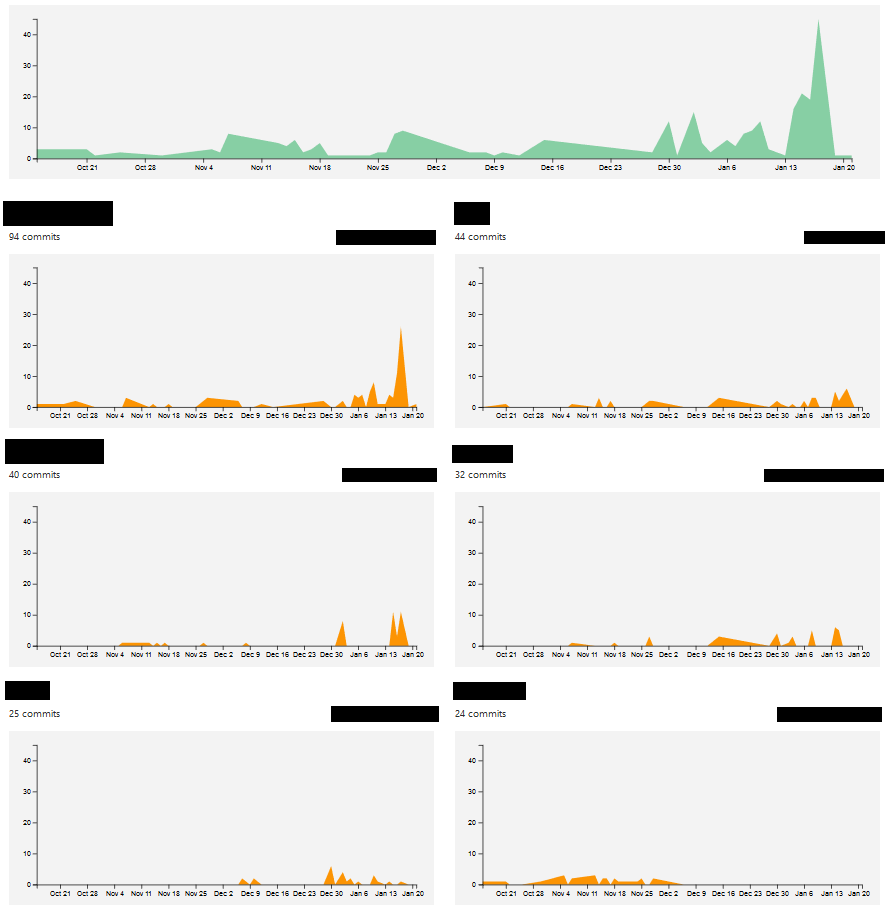
\includegraphics[scale=0.4]{slike/aktivnost.PNG} %veličina slike u odnosu na originalnu datoteku i pozicija slike
			\centering
			\caption{Primjer slike s potpisom}
			\label{fig:promjene}
		\end{figure}
		
		\begin{figure}[H]
			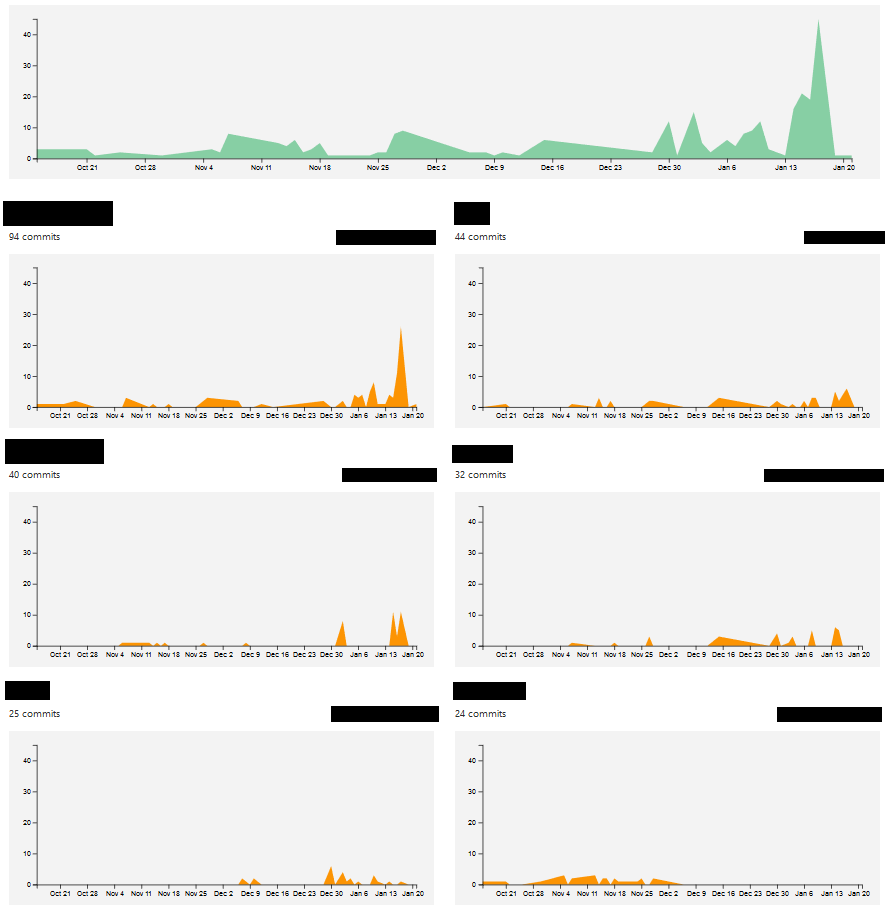
\includegraphics[width=\textwidth]{slike/aktivnost.PNG} %veličina u odnosu na širinu linije
			\caption{Primjer slike s potpisom 2}
			\label{fig:promjene2} %label mora biti drugaciji za svaku sliku
		\end{figure}
		
		Referenciranje slike \ref{fig:promjene2} u tekstu.
		
		\eject
		
	